% makeindex < aebpro_man.idx > aebpro_man.ind
\documentclass{article}
\usepackage[fleqn]{amsmath}
\usepackage[%
    web={centertitlepage,designv,
        forcolorpaper,latextoc,pro,useui},
    exerquiz,aebxmp
]{aeb_pro}
\usepackage{aeb_mlink}
\usepackage[altbullet]{lucidbry}
%\usepackage{myriadpro}

\usepackage{graphicx,array,longtable}
%\usepackage[usecmtt]{myriadpro}

%\def\uif#1{\textbf{\textsf{{#1}}}}
\let\uif\textsf

\newdimen\totaltextwidth
\totaltextwidth=\fullscreenwidth
\advance\totaltextwidth\oddsidemargin
\renewcommand{\webheadwrapper}[1]{%
    \hspace{-\oddsidemargin}%
    \makebox[\totaltextwidth][s]{#1}\hss
}

\setlongtables

\usepackage{acroman}

\usepackage[active]{srcltx}

\urlstyle{rm}

\newcommand{\prodName}{\textsf{PDF Flash Card}}
\newcommand{\sprodName}{\textsf{Flash Card}}
\newcommand{\ssprodName}{\textsf{Builder}}

\DeclareDocInfo
{
    university={\AcroTeX.Net},
    title={\prodName: Arithmetic},
    author={D. P. Story},
    email={dpstory@acrotex.net},
    subject={Documentation for AeB Exam Builder},
    talksite={\url{www.acrotex.net}},
    version={v1.0f, 2017/01/16},
    keywords={LaTeX, PDF, AcroTeX, PDF Flash Card, Arithmetic},
    copyrightStatus=True,
    copyrightNotice={Copyright (C) \the\year, D. P. Story},
    copyrightInfoURL={http://www.acrotex.net}
}

\renewcommand\hproportionwebtitle{.75}
\universityLayout{fontsize=Large,fontfamily=sffamily}
\titleLayout{fontsize=LARGE,fontfamily=sffamily}
\authorLayout{fontsize=Large,fontfamily=sffamily}
\tocLayout{fontsize=Large,color=aeb,fontfamily=sffamily}
\sectionLayout{indent=-62.5pt,fontsize=large,color=aeb,fontfamily=sffamily}
\subsectionLayout{indent=-31.25pt,color=aeb,fontfamily=sffamily}
\subsubsectionLayout{indent=0pt,color=aeb,fontfamily=sffamily}
\subsubDefaultDing{\texorpdfstring{$\bullet$}{\textrm\textbullet}}

\def\verygoodbreak{%
\vskip0pt plus1in\goodbreak\vskip0pt plus-1in}

\hyphenation{Java-Script}

\def\AcroT{Acro\!\TeX}\def\cAcroT{{\textcolor{blue}{\AcroT}}}
\def\AcroEB{\AcroT{} eDucation Bundle}\def\cAcroEB{\textcolor{blue}{\AcroEB}}
\def\AcroB{\AcroT{} Bundle}\def\cAcroB{\textcolor{blue}{\AcroB}}
\def\bUrl{http://www.math.uakron.edu/~dpstory}

\makeatletter
\let\bslash=\@backslashchar
\renewcommand{\paragraph}{\@startsection{paragraph}{4}{0pt}{6pt}{-3pt}{\bfseries}}

% Begin definition of \appendixsubsection
\newcounter{appendixsubsection} %\setcounter{appendixsubsection}{0}
\def\theappendixsubsection{\Alph{appendixsubsection}}
\def\theHappendixsubsection{\Alph{appendixsubsection}}
\newcommand\appendixsubsection{%
   \renewcommand{\@seccntformat}[1]{\csname the##1\endcsname.\enspace}%
   \@startsection{appendixsubsection}{1}{\z@}%
   {-2.5ex\@plus -1ex \@minus -.2ex}%
   {1ex \@plus .2ex}%
   {\normalfont\normalsize\bfseries\color{blue}}}
\let\appendixsubsectionmark=\@gobble
\expandafter\def\csname toclevel@appendixsubsection\endcsname{1}

\let\l@appendixsubsection=\l@section
\def\web@appendixsubsection#1#2#3{\web@parse#1\\\par\penalty-50 \hspace*{\@tempdima}\mbox{}%
        \textbf{\makebox[0pt][r]{\makebox[\@tempdima][r]{\hyperlink{#3}{\numberline.\enspace}}}\web@title}\endgraf}
% end definition of appendixsubsection

\makeatother

\hypersetup{linktocpage}

%\newenvironment{sverbatim}
%{\par\footnotesize\verbatim}{\endverbatim}

%\newcommand\redpoint{\par\ifdim\lastskip>0pt\relax\vskip-\lastskip\fi
%\vskip\medskipamount\noindent
% \makebox[\parindent][l]{\large\color{red}$\blacktriangleright$}}
%\newcommand\handpoint{\par\ifdim\lastskip>0pt\relax\vskip-\lastskip\fi
%\vskip\medskipamount\noindent
% \makebox[\parindent][l]{\large\color{blue}\ding{042}}}
%\newcommand\newtopic{\par\ifdim\lastskip>0pt\relax\vskip-\lastskip\fi
%\vskip\medskipamount\noindent
%}

\def\cs#1{\texttt{\bslash#1}}
\def\Cs#1{\hyperlink{#1}{\cs{#1}}}
\def\tableCs#1{\hyperlink{table#1}{\cs{#1}}}
\def\targ#1#2?{\hypertarget{#2}{\bslash#2}#1}

\def\dps{$\mbox{$\mathfrak D$\kern-.3em\mbox{$\mathfrak P$}%
   \kern-.6em \hbox{$\mathcal S$}}$}

\def\eForm{\textsf{eForm}}


\def\OpenToHere{\OpenAction{\JS{this.gotoNamedDest("Here")}}}
\def\OpenHere{\hypertarget{Here}{\strut}}%\OpenToHere

\nocopyright
\norevisionLabel
\makeatletter
%\let\web@copyright\@gobble
\let\web@revision\@gobble
\renewcommand\webdirectory
{%
    \par\ifeqforpaper\else\minimumskip\fi\vspace{\stretch{1}}%
    \begin{flushleft}\textbf{\large\web@directory}%
    \vspace{-3pt}
    \begin{itemize}\setlength{\itemsep}{-3pt}%
        \bfseries
        \item \leavevmode\hyperlink{webtoc}{\web@toc}%
        \item \web@article
        \item[] \rule[2pt]{2.25in}{.4pt}
        \item \textsf{\href{apb_man.pdf}{APB}} Documentation
        \item \href{webeqman.pdf}{\AcroEB} Documentation
    \end{itemize}
    \end{flushleft}
}
\renewcommand\titlepageTrailer
{%
    \webversion
%    \web@copyright\ \copyright\ \webcopyrightyears\ \webversion
        \hfill\url{http://www.acrotex.net}\\
    \web@revision\ \@date \hfill\href{mailto:\webemail}{\webemail}
}
\renewcommand\titlepageTrailer
{%
    \href{mailto:\webemail}{\webemail}
%    \web@copyright\ \copyright\ \webcopyrightyears\ \webversion
        \hfill\url{http://www.acrotex.net}\\
    \web@revision\ \@date \hfill\webversion
}
\makeatother

\newcounter{exampleno}
\def\theexampleno{\arabic{exampleno}}
\newcommand\Example{\refstepcounter{exampleno}%
\paragraph*{Example~\arabic{exampleno}.}}

\definecolor{aeb}{rgb}{0.24,0.38,0.68}%bleu
\universityColor{aeb}
\tocColor{aeb}

\everyCheckBox{\BC{.690 .769 .871}\BG{.941 1 .941}\textColor{1 0 0}}
\everyRadioButton{\BC{.690 .769 .871}\BG{.941 1 .941}\textColor{0 0 1}\symbolchoice{star}}

%\optionalPageMatter{%
%\begin{center}
%\hspace*{1in}\fbox{\begin{minipage}{.4\linewidth}\huge\bfseries
%Documentation still\\under construction
%\end{minipage}}
%\end{center}
%}


%\definePath\bgPath{"C:/Users/Public/Documents/ManualBGs/Manual_BG_Print_AeB.pdf"}
%\definePath\bgPath{"C:/Users/Public/Documents/ManualBGs/Manual_BG_Print_Games.pdf"}

\chngDocObjectTo{\newDO}{doc}
\begin{docassembly}
var titleOfManual="The fc_arith MANUAL";
var manualfilename="Manual_BG_Print_fetchbib.pdf";
var manualtemplate="Manual_BG_Brown.pdf"; // Blue, Green, Brown
var _pathToBlank="C:/Users/Public/Documents/ManualBGs/"+manualtemplate;
var doc;
var buildIt=false;
if ( buildIt ) {
    console.println("Creating new " + manualfilename + " file.");
    doc = \appopenDoc({cPath: _pathToBlank, bHidden: true});
    var _path=this.path;
    var pos=_path.lastIndexOf("/");
    _path=_path.substring(0,pos)+"/"+manualfilename;
    \docSaveAs\newDO ({ cPath: _path });
    doc.closeDoc();
    doc = \appopenDoc({cPath: manualfilename, oDoc:this, bHidden: true});
    f=doc.getField("ManualTitle");
    f.value=titleOfManual;
    doc.flattenPages();
    \docSaveAs\newDO({ cPath: manualfilename });
    doc.closeDoc();
} else {
    console.println("Using the current "+manualfilename+" file.");
}
var _path=this.path;
var pos=_path.lastIndexOf("/");
_path=_path.substring(0,pos)+"/"+manualfilename;
\addWatermarkFromFile({
    bOnTop:false,
    bOnPrint:false,
    cDIPath:_path
});
\executeSave();
\end{docassembly}
\begin{document}

\maketitle


\selectColors{linkColor=black}

\tableofcontents

\selectColors{linkColor=webgreen}


\section{Introduction}

The \textsf{fc\_arith} package is used to create an electronic ``flash card'' used to drill a student on elementary arithmetic, addition, subtraction, multiplication, and division. There are options for setting the range of the numbers to be used to randomly select numbers that appear in the arithmetic problem. Numbers can be set to 0, 1, or 2 decimal places. There is an optional timing mechanism that can be used to test a student's quickness in solving problems. There is a collection of fields used to tally the student's work on the arithmetic problems.

\paragraph*{History.} This is a re-work of an earlier PDF on drilling arithmetic problems. At that time, I took a blank PDF page and used the user interface of Acrobat to build the flash card.

In this version, I've taken the original flash card and developed a {\LaTeX} package for generating the flash card, added a number of customization options, and many other enhancements.

\begin{figure}[htb]
\begin{center}\setlength{\fboxsep}{0pt}
\fbox{\includegraphics[scale=.9]{graphics/fc04_a}}\\
\caption{\prodName: Arithmetic}\label{fcaritha}
\end{center}
\end{figure}

\section{Requirements and Options}

In this section, we review the requirements to build your own custom
flash card, and describe the package options available.

\subsection{Requirements}

The package is designed to be used with either a \textsf{Acrobat Distiller}
or a \textsf{pdflatex} workflow. The only true requirements are
\begin{itemize}
\item The \textsf{eforms} package (version 2.5c or later, 2010/03/21 or
later), a package distributed with AeB (the {Acro\!\TeX} eDucation Bundle%
\footnote{\url{http://www.math.uakron.edu/~dpstory/webeq.html}}

\item The \textsf{popupmenu} package
    \footnote{\url{http://mirror.ctan.org/macros/latex/contrib/popupmenu/}}
    which creates a menu system.

\end{itemize}

\redpoint Sample files: \texttt{fc-acrobat.tex} and \texttt{fc-noacrobat.tex}.

\newtopic\noindent I recommend the use of the \textsf{web} package to design your
page, just as the sample files do. Enhancements include the use of the
\textsf{aeb\_pro} package; see the sample file \texttt{fc-acrobat.tex} for an
illustration of the use of \textsf{aeb\_pro}.

\subsection{PDF Creators}

Any of the PDF creators used by the {\LaTeX} community
(\app{dvips/Distiller}, \app{pdflatex}, \app{lualatex}, and \app{xelatex})
may be used to build a {\prodName} document, as is demonstrated by the sample files
\texttt{fc-acrobat.tex} and \texttt{fc-noacrobat.tex}. Users who prefer
\app{pdflatex}, \app{lualatex}, and \app{xelatex} but own the \app{Acrobat}
application may want to look at the sample file \texttt{fc-acrobat.tex}.

\subsection{Options}

\begin{enumerate}

\item\texttt{allownegsub}: The original arithmetic flash card did not allow
    a negative difference, if this option is used, the differences are
    allowed to be negative. The default is to not to allow negative
    differences.

\item \texttt{nomenu}: There is a menu, labeled \uif{Settings},
    that allows the user change the range of the numbers generated by the
    flash card, set the number of decimal places, allows the user to toggle
    the \uif{Keypad} on and off, and so on. For further details
    see \Nameref{settings}.

     If this option is used, the menu does not appear. The default is for it to appear.

\item \texttt{showkeypadlink}: The \texttt{showkeypadlink} option generates
    a link with a label of \uif{Toggle Keypad} just above the
    keypad. Clicking the link toggles the visibility of the keypad.

    This option is useful if the \texttt{nomenu} option is taken, but
    you want the keypad available to users.

\item \texttt{operations}: Gives the ability to declare what operations
    flash card should show. Supported operations are \texttt{add},
    \texttt{sub}, \texttt{mul}, \texttt{div}. For example,
\begin{Verbatim}[xleftmargin=\amtIndent]
operations={add,sub}
\end{Verbatim}
    creates a flash card in which only addition and subtraction problems
    are available.

    The default is to make available all operations.


\item \texttt{notimedscores}: As can be seen in
    \hyperref[fcaritha]{Figure~\ref*{fcaritha}}, page~\pageref*{fcaritha},
    the flash card has many fields that key of the user's performance. One
    of these is the \uif{Timed Scores} row; this row gives a
    score based on time required to answer the problem correctly. Some
    teachers may not want such pressure placed on their students, so if
    this option is taken, the row is not generated.

\end{enumerate}

\section{The Components of the \sprodName}

We describe the elements of the flash card as they appear, from top to
bottom, in \hyperref[fcaritha]{Figure~\ref*{fcaritha}},
page~\pageref*{fcaritha}.

\subsection{Settings}\label{settings}

The \uif{Settings} menu, which can be removed with the
\texttt{nomenu} option, consists of five menu items:
\uif{Options}, \uif{Toggle Keypad},
\uif{Mouse Friendly Keypad}, \uif{Touch Friendly
Keypad}, and \uif{About PDF Flash Cards}, see the figure below.

\begin{figure}[htb]
\begin{center}\setlength{\fboxsep}{0pt}
\fbox{\includegraphics[scale=.75]{graphics/menu_settings}}\\
\caption{The \texorpdfstring{\protect\uif{Settings}}{Settings} menu}\label{menuSettings}
\end{center}
\end{figure}

The labeling for the \uif{Settings} menu is modified using the
command \cs{fcSettings}, the default definition is
\verb!\newcommand{\fcSettings}{Settings}!. The color of the link is set by
the command \cs{fcSettingsColor}, the default definition of which is
\verb!\newcommand{\fcSettingsColor}{black}!.

\paragraph*{The \env{MenuFC} environment.} The \uif{Settings} menu is created by the environment seen below and found the
the demonstration files of this distribution. The \env{MenuFC} is a special environment
defined in \pkg{fc\_arith} to enclose the menu items.
\begin{Verbatim}[xleftmargin=\amtIndent]
\begin{MenuFC}
    \fcOptionsMenuItem
    \fcToggleKeypadMenuItem
    \fcMouseKPMenuItem
    \fcTouchKPMenuItem
    \fcAboutFC
\end{MenuFC}
\end{Verbatim}
You can exclude some of the menu items listed above. From
Figure~\ref{menuSettings}, the \uif{Mouse Friendly Keypad} and
\uif{Touch Friendly Keypad} items are initially grayed out. They
become active when \uif{Toggle Keypad} is selected. The
\uif{Touch Friendly Keypad} is larger than the
\uif{Mouse Friendly Keypad} and fits fat fingers better. See
\mlNameref{toggleKp} for additional information on the keypad.

The names of the menu items may be localized to your own language.
\begin{Verbatim}[xleftmargin=\amtIndent]
\renewcommand\fcOptionsMenuItemTitle{Options}
\renewcommand\fcToggleKeypadMenuItemTitle{Toggle Keypad}
\renewcommand\fcMouseKPMenuItemTitle{Touch Friendly Keypad}
\renewcommand\fcTouchKPMenuItemTitle{Mouse Friendly Keypad}
\renewcommand\fcAboutFCTitle{About PDF Flash Cards}
\end{Verbatim}
The default English title defines are shown. All can be redefined in the preamble or in the
customization file \texttt{fc\_custom.def}, discussed in \hyperref[s:CusStrs]{Section~\ref*{s:CusStrs}}.

\subparagraph*{Adding custom menu items.} You can also add custom menu items,
but some effort. Suppose we want to add an item titled \uif{AcroTeX.Net}. The
special environment generates a \env{popupmenu} environment, as defined by
the \pkg{popupmenu} package. We use the \cs{item} command, as defined within
a \env{popupmenu} environment and assign values for \texttt{title} and
\texttt{return}. The value of \texttt{return} is any string, but
\pkg{fc\_arith} puts a restriction on its value: it must not be 0, 1, 2, 3,
or 4, for these values are used by the preexistent menu items.
\begin{Verbatim}[xleftmargin=\amtIndent]
\begin{MenuFC}
    \fcOptionsMenuItem
    \fcToggleKeypadMenuItem
    \fcMouseKPMenuItem
    \fcTouchKPMenuItem
    \item{title=AcroTeX.Net Home,return=acrotexhome}
    \item{title=AcroTeX.Net Blog,return=acrotexblog}
    \fcAboutFC
\end{MenuFC}
\end{Verbatim}
The \env{MenuFC} environment occurs in the preamble of your document. Then to associate an action
with the use selecting this new item, add the following code to the preamble as well:
\begin{Verbatim}[xleftmargin=\amtIndent]
\begin{insDLJS}{cmfc}{Custom Menu Events}
function processCustomFcMenu(n) {
    // n=the return value of the selected item
    switch(n) {
        case "acrotexhome":
            app.launchURL("http://www.acrotex.net",false);
            break;
        case "acrotexblog":
            app.launchURL("http://blog.acrotex.net",false);
            break;
    }
}
\end{insDLJS}
\end{Verbatim}
Here I use the JavaScript \texttt{switch} operator to take the incoming
argument \texttt{n} (the return value) and associating an action. If the
user-defined \texttt{processCustomerFcMenu()} is created, \pkg{fc\_arith}
passes the code scream from the function \texttt{processFcMenu()}, which
handles all the predefined menu items, to \texttt{processCustomerFcMenu()}.

With these definitions, when the user selects `\uif{AcroTeX.Net Home}', the
default browser opens and loads the page \url{http://www.acrotex.net}. This
technique is illustrated in the file \texttt{fc\_noacrobat.tex}.



\subsubsection{Options}\label{options}

The \uif{Options} menu item calls forth the
\uif{Options} dialog box,
\hyperref[menuOptions]{Figure~\ref*{menuOptions}},
page~\pageref*{menuOptions}. Through this dialog box, you can set the
intervals from which random numbers are drawn, and their precision.

\paragraph*{Addition, Subtraction, Multiplication.} We handle these three
operations in the same way, so we explain them together. For these three
we have a top number and a bottom number.
\begin{quote}%\large
\begin{tabular}{rc@{ }rc@{ }rc@{ }r}
top & & $14$ & & $17$ & & $12$ \\
bottom &$+$& $2$ &$-$& $4$ &$\times$& $7$ \\
\end{tabular}
\end{quote}
In the dialog box, you can set the range (the interval) of numbers from which
randomly generated numbers are taken. For example, the
\hyperref[menuOptions]{Figure~\ref*{menuOptions}} on
page~\pageref*{menuOptions} specifies that for \textsf{Addition} problems, the top
value should come from a range of $2$ to $20$, the bottom range is $5$ to
$30$, and there should be no decimal places (hence, for this example, we
deal with integer arithmetic). {\prodName} supports at most two decimal places.

\begin{figure}[htb]
\begin{center}\setlength{\fboxsep}{0pt}
\fbox{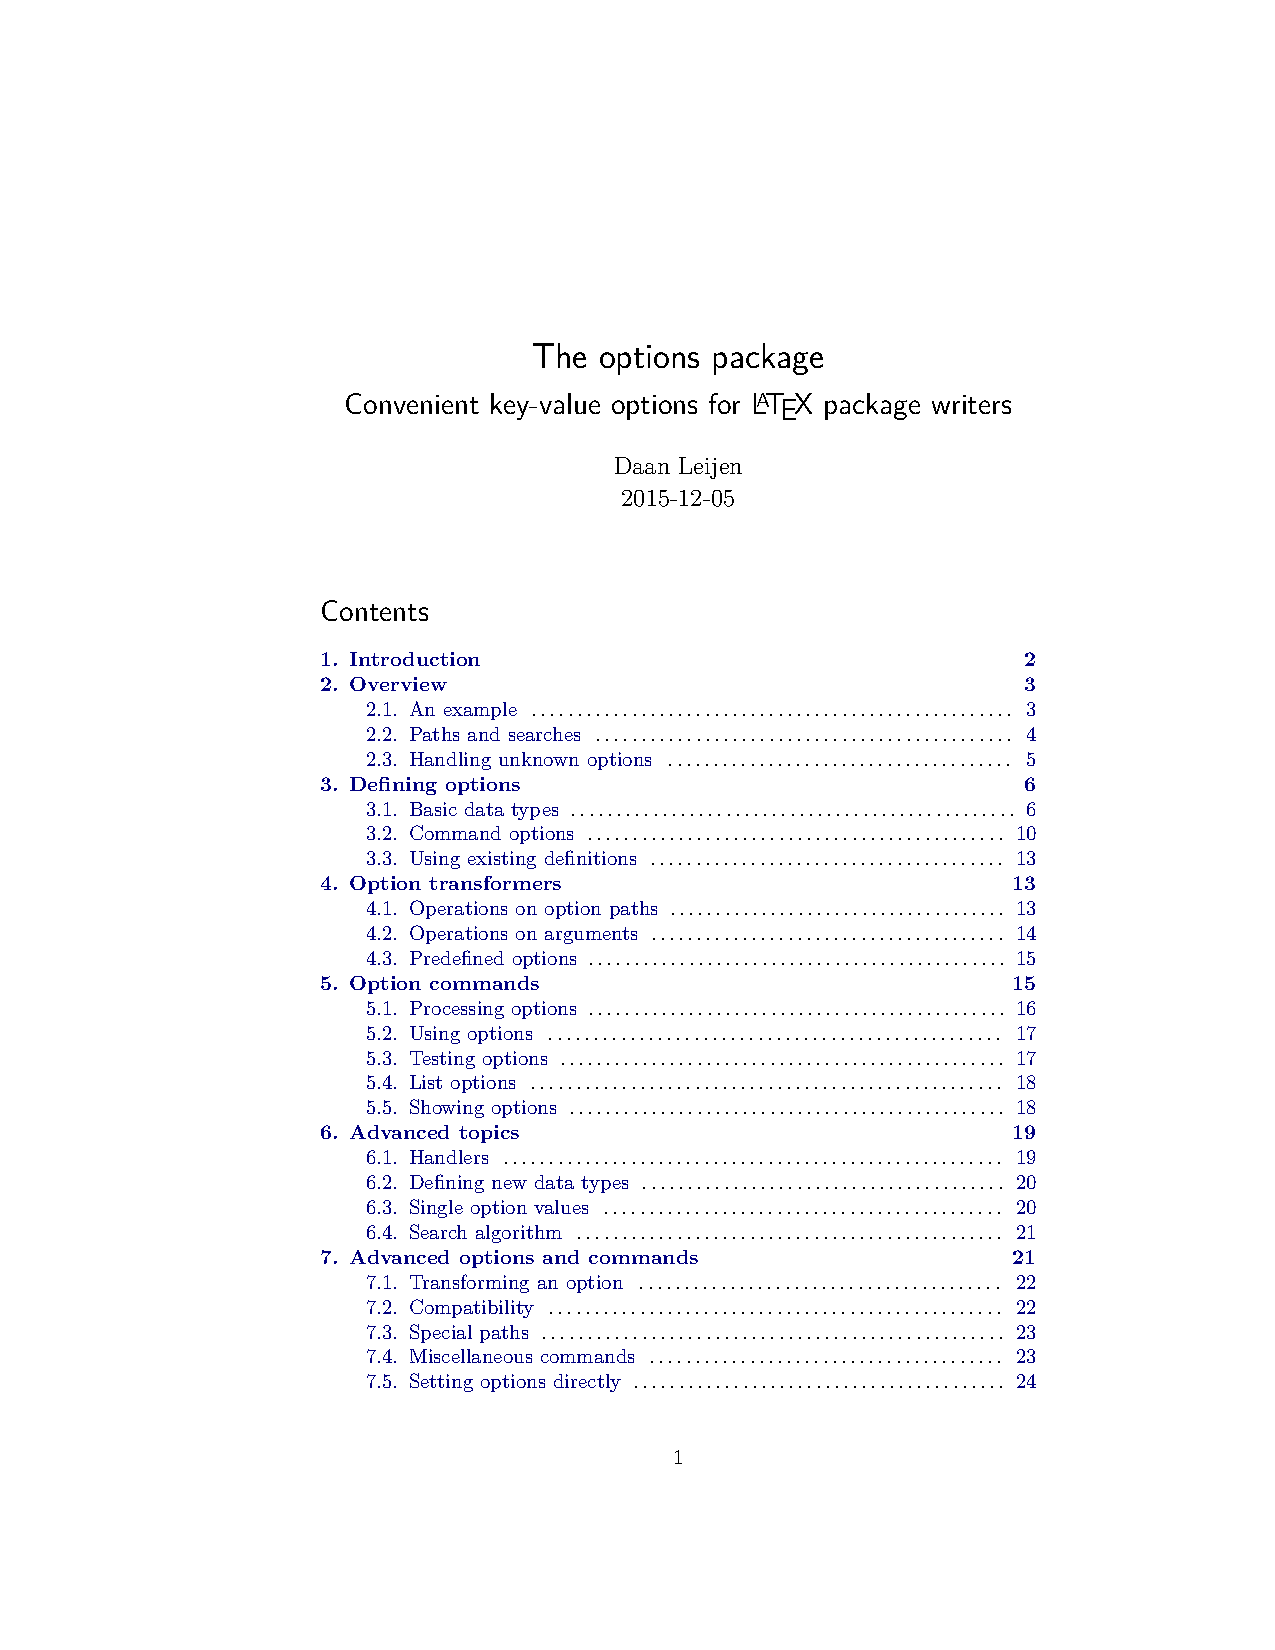
\includegraphics[scale=.75]{graphics/options}}\\
\caption{The \texorpdfstring{\protect\uif{Options}}{Options} dialog box}\label{menuOptions}
\end{center}
\end{figure}

\paragraph*{Division.} Division is handled separately because of the way the
problem is generated. Rather than randomly generating the top and bottom
values as is done for addition, subtraction, and multiplication, the
\textsf{fc\_arith} package randomly generates the \emph{quotient} and
\emph{divisor}, then calculates the dividend
\begin{equation*}
    \text{dividend}=\text{quotient}\times\text{divisor}
\end{equation*}
This leads to the assurance of a clean division problem with no nasty
rounding, or infinite decimal expansions ($ 1/3 0.33333\dots $). It is a
design decision made for the original \prodName, where the targeted audience was
elementary school age students.

The top is now the dividend and the bottom is the divisor, but in the
\uif{Options} dialog box, \uif{Range Top} and
\uif{Range Bottom} is replaced by \uif{Range
Quotient} and \uif{Range Divisor} to reflect the different way
of generating the division problem.

\redpoint The dialog box retains the settings only during the current session
of Adobe Reader. The Reader does not have the ability to save data so once
the {\sprodName} is closed, the data is lost.

\subsubsection{Toggle Keypad}\label{toggleKp}

Selecting the \uif{Toggle Keypad} submenu item toggles the
keypad, which is initially hidden, see
\hyperref[menuKeypad]{Figure~\ref*{menuKeypad}}. The keyboard input region is
changed to read only, the student can only enter through the keypad.

The touch friendly keypad is larger by an amount of 5 points. This can be changed
if you feel the touch friendly is not large enough by the command \cs{amtChngMouToTou}.
\begin{Verbatim}[xleftmargin=\amtIndent]
\newcommand\amtChngMouToTou{5}
\end{Verbatim}
The default definition is given above, use \cs{renewcommand} to change this,
keeping in mind a larger keypad may go beyond the page. Some positioning
adjustments may be needed.

\begin{figure}[htb]
\begin{center}\setlength{\fboxsep}{0pt}
\fbox{\includegraphics[scale=1]{graphics/keypad}}\\
\caption{The \texorpdfstring{\protect\uif{Keypad}}{Keypad}}\label{menuKeypad}
\end{center}
\end{figure}

\subsubsection{About PDF Flash Card}\label{aboutFC}

Some information about the {\prodName}.

\subsection{The \texorpdfstring{\protect\cs{arithProb}}
{\CMD{arithProb}} Command}

The \cs{arithProb} command is a trio of form fields laid out to display an
arithmetic problem, see
\hyperref[arithprob]{Figure~\ref*{arithprob}},\begin{NoHyper}\footnote{Figure~\ref*{arithprob}
shows an outline of the fields so you can see their relative
positions.}\end{NoHyper} and \hyperref[fcannot]{Figure~\ref*{fcannot}},
page~\pageref*{fcannot}.

\begin{figure}[htb]
\begin{center}\setlength{\fboxsep}{0pt}
\fbox{\includegraphics[scale=1]{graphics/arithprob}}\\
\caption{The \cs{arithProb} Command}\label{arithprob}
\end{center}
\end{figure}

The three fields and their descriptions follow:
\begin{itemize}
    \item \texttt{top}: The name of this text field is \texttt{top}, and it
        holds the upper most number in the problem (this number is called
        by different names depending on the operation, we'll just call it
        the top number).
    \item \texttt{bottom}: The name of this text field is \texttt{bottom},
        and it holds the lower number in the problem.
    \item \texttt{operation}: The name of this text field is
        \texttt{operation}.
\end{itemize}
The top and bottom fields use a monospace font (courier-bold) so that when
there are decimal numbers involved, the numbers will align properly.

\begin{figure}[htb]
\begin{center}\setlength{\fboxsep}{0pt}
\fbox{\includegraphics[scale=.5]{graphics/fc_annot}}\\
\caption{The \prodName, Annotated}\label{fcannot}
\end{center}
\end{figure}



\paragraph*{Appearance Parameters for \cs{arithProb}.} The three fields are
bundled together as a unit, which makes it difficult to set the appearance of
each individual field, unless you want to redefine \cs{arithProb}. There are,
however, several commands available to make some adjustments to meet your
needs.
\begin{itemize}
    \item \cs{tBGNoBorder}: This is a command that holds various
        \textsf{eform} key-value pairs that are passed to these three
        fields. The default definition of \cs{tBGNoBorder} is
\begin{Verbatim}[xleftmargin=\amtIndent]
\newcommand{\tBGNoBorder}{\BC{}\BG{}\autoCenter{n}
    \textSize{0}\textColor{1 0 0}\Ff\FfReadOnly}
\end{Verbatim}
    This set of parameters gives a field with transparent border and
    background, auto-adjusting font size, red text, and with a readonly
    attribute. This command can be redefined.
    \item \cs{monoSpaceFont}: These three fields use a monospace font, you
        can change this font using \cs{monoSpaceFont}. The default
        definition is
\begin{Verbatim}[xleftmargin=\amtIndent]
\newcommand{\monoSpaceFont}{CoBo}
\end{Verbatim}
    which is courier-bold.
    \item \cs{setDimOf}: The \cs{setDimOf} can be used to set the
        dimensions of these fields. The command takes three parameters,
        field name, width and height. The default definitions for these
        three fields are
\begin{Verbatim}[xleftmargin=\amtIndent]
\setDimOf{top}{1in}{0.62in}
\setDimOf{operation}{.38in}{.62in}
\setDimOf{bottom}{1in}{0.62in}
\end{Verbatim}
Note that the dimensions of \texttt{top} and \texttt{bottom} are the same,
as they are supposed to align vertically.
\end{itemize}

\subsection{The \texorpdfstring{\protect\cs{inputRegion}} {\CMD{inputRegion}} Command}

When the keypad field is hidden (see the \Nameref{keypad}), the user inputs
the response to the arithmetic problem into the field titled \texttt{result}.
This field is placed on the flash card using the \cs{inputRegion} command;
this field is usually placed immediately beneath the \cs{arithProb} command
so that the \texttt{result} field is aligned vertically with the \texttt{top}
and \texttt{bottom} fields.

The syntax for \cs{inputRegion} is
\begin{Verbatim}[xleftmargin=\amtIndent,commandchars=!()]
\inputRegion[!ameta(eform_parameters)]
\end{Verbatim}
The default appearance properties are pre-defined as
\begin{Verbatim}[xleftmargin=\amtIndent]
\newcommand{\cBGNoBorder}{\Q{1}\BC{}\BG{}\autoCenter{n}
    \textSize{0}\textColor{0 0 0}\BG{.75 .75 .75}
    \Ff\FfReadOnly}
\end{Verbatim}
You can redefine \cs{cBGNoBorder}, or you can introduce a few changes through
the optional parameter.

The dimensions of the \texttt{result} fields can be set using \cs{setDimOf}.
The default definition is
\begin{Verbatim}[xleftmargin=\amtIndent]
\setDimOf{result}{1.38in}{0.62in}
\end{Verbatim}
The \texttt{0.62in} is the same width used for the \texttt{top} and \texttt{bottom} fields.

\subsection{The \texorpdfstring{\protect\cs{startAgain}}{\CMD{startAgain}}
    and \texorpdfstring{\protect\cs{newCard}} {\CMD{newCard}} Command}\label{startAgainnewCard}

The \cs{newCard} command generates a push button named \texttt{NewProblem},
when pushed, a new arithmetic is randomly generated. The \cs{startAgain}
command creates a push button named \texttt{StartAgain}, when pushed, all
fields are cleared, and any JS variables are re-initialized. The syntax for
these two fields is
\begin{Verbatim}[xleftmargin=\amtIndent,commandchars=!()]
\startAgain[!ameta(eform_parameters)]
\newCard[!ameta(eform_parameters)]
\end{Verbatim}
The default appearance properties are pre-defined as
\begin{Verbatim}[xleftmargin=\amtIndent]
\newcommand{\tBGNoBorderI}{\BC{}\BG{}\autoCenter{n}
    \textSize{0}\textColor{1 0 0}}
\end{Verbatim}
You can redefine \cs{tBGNoBorderI}, or you can introduce a few changes
through the optional parameter.

The dimensions of \texttt{NewProblem} and \texttt{StartAgain} can be set
using \cs{setDimOf}. The default definition is
\begin{Verbatim}[xleftmargin=\amtIndent]
\setDimOf{StartAgain}{0.88in}{0.62in}
\setDimOf{NewProblem}{0.88in}{0.62in}
\end{Verbatim}
The text font used by these two fields is determined by the command
\cs{fieldFont}. The default definition of \cs{fieldFont} is
\begin{Verbatim}[xleftmargin=\amtIndent]
\newcommand{\fieldFont}{Helv}
\end{Verbatim}
The name for the font should be one of the 13 basic fonts, or a PostScript
font. In the latter case, most likely, the Acrobat Distiller is needed for
PDF creation.

\subsection{The \texorpdfstring{\protect\cs{alertbox}}{\CMD{alertbox}} Command}\label{alertbox}

The \cs{alertbox} command creates a transparent text field named
\texttt{alertbox}, which displays \uif{Right!} and \uif{Wrong!}
messages. The syntax for this field is
\begin{Verbatim}[xleftmargin=\amtIndent,commandchars=!()]
\alertbox[!ameta(eform_parameters)]
\end{Verbatim}
The default appearance properties are pre-defined as
\begin{Verbatim}[xleftmargin=\amtIndent]
\newcommand{\tBGNoBorder}{\BC{}\BG{}\autoCenter{n}
    \textSize{0}\textColor{1 0 0}\Ff\FfReadOnly}
\end{Verbatim}
You can redefine \cs{tBGNoBorder}, or you can introduce a few changes through
the optional parameter.

The dimensions of \texttt{alertbox} can be set using \cs{setDimOf}. The default definition is
\begin{Verbatim}[xleftmargin=\amtIndent]
\setDimOf{alertbox}{.88in}{.62in}
\end{Verbatim}

\subsection{The \texorpdfstring{\protect\cs{Keypad}}{\CMD{Keypad}} Command}\label{keypad}

The \cs{Keypad} creates a number of fields in the form of a keypad, see
\hyperref[keypad]{Figure~\ref*{keypad}}. When the keypad is visible, the
result field (created by \cs{inputRegion}) is read-only.

\begin{figure}[htb]
\begin{quote}
\settowidth{\totaltextwidth}{Figure 0: The Keypad}
\begin{minipage}{\totaltextwidth}\centering
\setlength{\fboxsep}{0pt}
\fbox{\includegraphics[scale=.6]{graphics/keypad}}\\
\caption{The Keypad}\label{keypad}
\end{minipage}
\end{quote}
\end{figure}

\newtopic\noindent
The default appearance properties are pre-defined as
\begin{Verbatim}[xleftmargin=\amtIndent]
\newcommand{\tBGNoBorder}{\BC{}\BG{}\autoCenter{n}
    \textSize{0}\textColor{1 0 0}\Ff\FfReadOnly}
\end{Verbatim}
You can redefine \cs{tBGNoBorder}, or you can introduce a few changes through the optional parameter.

The dimension of each key is based on the value of \cs{szNum}, the default definition is
\begin{Verbatim}[xleftmargin=\amtIndent]
\newcommand{\szNum}{14bp}
\end{Verbatim}
The default appearance properties are pre-defined as
\begin{Verbatim}[xleftmargin=\amtIndent]
\newcommand{\myNumPadI}{\F\FHidden\autoCenter{n}
    \textSize{8}\textFont{\fieldFont}\S{S}}
\end{Verbatim}
You can redefine \cs{myNumPadI}.

The labeling for the \uif{Enter} and \uif{Back} keys can be redefined as well, their definitions are
\begin{Verbatim}[xleftmargin=\amtIndent]
\newcommand{\kpBack}{Back}
\newcommand{\kpEnter}{Enter}
\end{Verbatim}

\subsection{The \texorpdfstring{\protect\cs{cbTiming}}{\CMD{cbTiming}} Command}\label{cbTiming}

The \cs{cbTiming} command creates a combo box, named \texttt{TimeDelay}, that
lists a menu of time values for the user to practice against. The default is
\uif{No Timing}.

\paragraph*{Rules for Timed Responses.} When \uif{No Timing} is in effect,
if the student correctly answers the problem in the time allotted, credit is
awarded; otherwise, no credit is given. When another time setting is in
effect, the same rule applies as above, except no credit is awarded if the
time is up, even if the response is correct. Click on the push button labeled
\uif{Timed Scores} to see the rules for awarding the points, depicted in Figure~\ref*{fig:timedscores}.

\begin{figure}[htb]\centering
\setlength{\fboxsep}{0pt}
\fbox{\includegraphics[scale=.6]{graphics/timedscores}}\\
\caption{The timed scores dialog box}\label{fig:timedscores}
\end{figure}

The strings of this dialog box may be localize to another language, refer to \hyperref[s:CusStrs]{Section~\ref*{s:CusStrs}}
for details.

\newtopic\noindent\textbf{Note:} The original idea behind the timed scores is to have
students compete against each other. For example, for addition, let each
student attempt $10$ problems, the highest score wins! Try this with
\uif{No Timing} first, then start decreasing the time value
progressively down to $5\,\text{sec}$. Who is the fastest with the mostest!

The syntax for \cs{cbTiming} is
\begin{Verbatim}[xleftmargin=\amtIndent,commandchars=!()]
\cbTiming[!ameta(eform_parameters)]
\end{Verbatim}
The default appearance properties are pre-defined as
\begin{Verbatim}[xleftmargin=\amtIndent]
\newcommand{\cBGBorder}{\BC{0 0 0}\BG{.75 .75 .75}
    \autoCenter{n}\textSize{0}\textColor{0 0 0}}
\end{Verbatim}
You can redefine \cs{cBGBorder}, or you can introduce a few changes through
the optional parameter.

The dimensions of \texttt{TimeDelay} field can be set using \cs{setDimOf}:
\begin{Verbatim}[xleftmargin=\amtIndent]
\setDimOf{TimeDelay}{0.9in}{0.24in}
\end{Verbatim}
The font used in the list box is determined by the value of \cs{fieldFont},
the default definition is \verb!\newcommand{\fieldFont}{Helv}!.

The string \uif{No Timing} can be modified using \cs{fcNoTiming}:
\begin{Verbatim}[xleftmargin=\amtIndent]
\newcommand{\fcNoTiming}{No Timing}
\end{Verbatim}


\subsection{The \texorpdfstring{\protect\cs{ansField}}{\CMD{ansField}} Command}\label{ansField}

The \cs{ansField} creates a text field named \texttt{ansregion}; the field
holds the correct answer to the problem.

The syntax for \cs{cbTiming} is
\begin{Verbatim}[xleftmargin=\amtIndent,commandchars=!()]
\ansField[!ameta(eform_parameters)]
\end{Verbatim}
The appearance of this field can be modified using \cs{cBGNoBorder}; the default definition is,
\begin{Verbatim}[xleftmargin=\amtIndent]
\newcommand{\cBGNoBorder}{\Q{1}\BC{}\BG{}\autoCenter{n}
    \textSize{0}\textColor{0 0 0}\BG{.75 .75 .75}\Ff\FfReadOnly}
\end{Verbatim}
This can be redefined as desired.

The dimensions of \texttt{ansregion} can be set be \cs{setDimOf}:
\begin{Verbatim}[xleftmargin=\amtIndent]
\setDimOf{ansregion}{.87in+10bp}{.24in}
\end{Verbatim}
Notice that a little arithmetic on dimensions is used, this is because the
\textsf{fc\_arith} package inputs the \textsf{calc} package.

The \texttt{ansregion} has a formatting string, it prepends \texttt{Answer:}
to the correct answer. You can change this word using the command
\cs{fmtAnswer} the definition of which is
\begin{Verbatim}[xleftmargin=\amtIndent]
\newcommand{\fmtAnswer}{Answer:}
\end{Verbatim}

\subsection{The \texorpdfstring{\protect\cs{cbOperation}}{\CMD{cbOperation}} Command}\label{cbOperation}

The \cs{cbOperation} command creates a combo box, named
\texttt{ChooseOperation}, that lists a menu of arithmetic operations for the
user to select.

The syntax for \cs{cbOperation} is
\begin{Verbatim}[xleftmargin=\amtIndent,commandchars=!()]
\cbOperation[!ameta(eform_parameters)]
\end{Verbatim}
The default appearance properties are pre-defined as
\begin{Verbatim}[xleftmargin=\amtIndent]
\newcommand{\cBGBorder}{\BC{0 0 0}\BG{.75 .75 .75}
    \autoCenter{n}\textSize{0}\textColor{0 0 0}}
\end{Verbatim}
You can redefine \cs{cBGBorder}, or you can introduce a few changes through
the optional parameter.

The dimensions of \texttt{ChooseOperation} field can be set using \cs{setDimOf}:
\begin{Verbatim}[xleftmargin=\amtIndent]
\setDimOf{ChooseOperation}{1.38in-10bp}{0.24in}
\end{Verbatim}
The font used in the list box is determined by the value of \cs{fieldFont},
the default definition is \verb!\newcommand{\fieldFont}{Helv}!.

The strings used in the combo box can be modified by redefining the following commands:
\begin{Verbatim}[xleftmargin=\amtIndent]
\newcommand{\fcAddition}{Addition}
\newcommand{\fcSubtraction}{Subtraction}
\newcommand{\fcMultiplication}{Multiplication}
\newcommand{\fcDivision}{Division}
\end{Verbatim}

\subsection{The \texorpdfstring{\protect\cs{statsFields}}{\CMD{statsFields}} Command}\label{statsFields}

The \cs{statsField} command creates a number of fields that hold the
statistics of the user's attempts at answering arithmetic problems.

The following definitions are used.
\begin{Verbatim}[xleftmargin=\amtIndent]
\setDimOf{fcSF}{0.37in}{0.25in}
\newcommand{\statsFieldOpColor}{1 0 0}
\newcommand{\statsFieldColor}{blue}
\end{Verbatim}
The first is to set the dimensions of each field, they all have the same
dimension. The second sets the color for the operations of $+$, $-$, $\times$
and \char247; the default color for the labeling of these operations is red
(\verb!{1 0 0}! in the RGB color space. The \cs{statsFieldColor} is a color
of typeset content and its default is \texttt{blue}. (\cs{statsFieldOpColor}
is used in form fields, while \cs{statsFieldColor} is {\LaTeX}ed.)

\section{Other Customizations}

In this section, we itemize various other customizations not already mentioned.

\subsection{Setting the Range and Decimal}

The command \cs{DeclareArithParams}---executed in the preamble only---is
used to set the start-up parameters of the \uif{Options} menu
\hyperref[menuOptions]{Figure~\ref*{menuOptions}} on
page~\pageref*{menuOptions}.\footnote{If the \texttt{nomenu} option is
taken, the parameters are still used, but user has no way of changing
them.}

The \cs{DeclareArithParams} takes a series of key-values. We classify the
keys by function: setting the intervals and setting the decimal places.
\begin{itemize}
    \item \textbf{Setting the intervals.} Each of these keys takes an
        interval of the form \texttt{[a,b]}. Because there is a comma in the
        interval notation, the interval needs to be enclosed in braces, like
        so \verb!{[a,b]}!.
    \begin{itemize}
        \item \textbf{Addition:} \verb!addT={[a,b]}!, \verb!addB={[a,b]}!
        \item \textbf{Subtraction:} \verb!subT={[a,b]}!, \verb!subB={[a,b]}!
        \item \textbf{Multiplication:} \verb!mulT={[a,b]}!, \verb!mulB={[a,b]}!
        \item \textbf{Division:} \verb!divQ={[a,b]}!, \verb!divB={[a,b]}!
    \end{itemize}
    \item {Setting the decimal places.} The value of these keys take any
        of three values \texttt{none}, \texttt{1}, or \texttt{2}. In all
        cases, the default is \texttt{none}.
    \begin{itemize}
        \item \textbf{Addition:} \verb!addDecT=none|1|2!, \verb!addDecB=none|1|2!
        \item \textbf{Subtraction:} \verb!subDecT=none|1|2!, \verb!subDecB=none|1|2!
        \item \textbf{Multiplication:} \verb!mulT=none|1|2!, \verb!mulDecB=none|1|2!
        \item \textbf{Division:} \verb!divDecQ=none|1|2!, \verb!divDecB=none|1|2!
    \end{itemize}
\end{itemize}

The default definitions are
\begin{Verbatim}[xleftmargin=\amtIndent]
\DeclareArithParams
{%
     addT={[0,100]},addB={[0,100]},
     subT={[0,100]},subB={[0,100]},
     mulT={[0,100]},mulB={[0,10]},
     divQ={[0,10]},divB={[0,10]},
}
\end{Verbatim}
The decimal points are all set to \texttt{none}, by default.

\newtopic\noindent Below is a complete example of setting all parameters.
\begin{Verbatim}[xleftmargin=\amtIndent]
\DeclareArithParams
{%
     addT={[2,20]},addB={[5,30]},
     addDecT=none,addDecB=2,
     subT={[1,5]},subB={[5,10]},
     subDecT=1,subDecB=2,
     mulT={[1,12]},mulB={[1,10]},
     mulDecT=1,mulDecB=2,
     divQ={[1,4]},divB={[1,10]},
     divDecQ=1,divDecB=2,
}
\end{Verbatim}

\subsection{Customization Strings}\label{s:CusStrs}

The following English strings are used in {\sprodName}. These can all be redefined.

\newtopic\noindent The following is a message that appears in an alert box when your time is up.
\begin{Verbatim}[xleftmargin=\amtIndent]
\newcommand{\timeUpMsg}{Your Time is UP!}
\end{Verbatim}
These next two are the default messages in the \texttt{alertbox} text field.
\begin{Verbatim}[xleftmargin=\amtIndent]
\newcommand{\rightMsg}{Right!}
\newcommand{\wrongMsg}{Wrong!}
\end{Verbatim}
The text on the \texttt{StartAgain} and \texttt{NewProblem}.
\begin{Verbatim}[xleftmargin=\amtIndent]
\newcommand{\startAgainMsg}{Start Again}
\newcommand{\newCardMsg}{New Card}
\end{Verbatim}
The formatting of the \texttt{ansfield}.
\begin{Verbatim}[xleftmargin=\amtIndent]
\newcommand{\fmtAnswer}{Answer:}
\end{Verbatim}
Labels that appear on the key pad.
\begin{Verbatim}[xleftmargin=\amtIndent]
\newcommand{\kpBack}{Back}
\newcommand{\kpEnter}{Enter}
\end{Verbatim}
The default setting for the \texttt{TimeDelay} combo box.
\begin{Verbatim}[xleftmargin=\amtIndent]
\newcommand{\fcNoTiming}{No Timing}
\end{Verbatim}
The listing of arithmetic operations in to combo box titled \texttt{ChooseOperation}.
\begin{Verbatim}[xleftmargin=\amtIndent]
\newcommand{\fcAddition}{Addition}
\newcommand{\fcSubtraction}{Subtraction}
\newcommand{\fcMultiplication}{Multiplication}
\newcommand{\fcDivision}{Division}
\end{Verbatim}
The text of the menu that, by default, appears in the upper left-corner.
\begin{Verbatim}[xleftmargin=\amtIndent]
\newcommand{\fcSettings}{Settings}
\renewcommand\fcOptionsMenuItemTitle{Options}
\renewcommand\fcToggleKeypadMenuItemTitle{Toggle Keypad}
\renewcommand\fcMouseKPMenuItemTitle{Touch Friendly Keypad}
\renewcommand\fcTouchKPMenuItemTitle{Mouse Friendly Keypad}
\renewcommand\fcAboutFCTitle{About PDF Flash Cards}
\end{Verbatim}
Some text strings that are part of the \cs{statsField} set.
\begin{Verbatim}[xleftmargin=\amtIndent]
\newcommand{\toggleKeypad}{Toggle Keypad}
\newcommand{\operation}{Operation}
\newcommand{\numCorrect}{Number Correct}
\newcommand{\numAttempted}{Number Attempted}
\newcommand{\percentCorrect}{Percentage Correct}
\newcommand{\timedScores}{Timed Scores}
\end{Verbatim}
Some strings in the timed scores dialog box (Figure~\ref{fig:timedscores}).
\begin{Verbatim}[xleftmargin=\amtIndent]
\def\fctCharWidth{22}
\def\fctInstr{"Points are awarded, based on time,
    for successfully solving a problem:"}
\def\fctTimeElapsed{"Time elapsed"}
\def\fctPoints{"Points"}
\def\fctLessThanV{"Less than 5 sec"}
\def\fctLessThanVPoints{6}
\def\fctBtwnVAndX{"Between 5 and 10 sec"}
\def\fctBtwnVAndXPoints{5}
\def\fctBtwnXAndXV{"Between 10 and 15 sec"}
\def\fctBtwnXAndXVPoints{4}
\def\fctBtwnXVAndXX{"Between 15 and 20 sec"}
\def\fctBtwnXVAndXXPoints{3}
\def\fctBtwnXXAndXXV{"Between 20 and 25 sec"}
\def\fctBtwnXXAndXXVPoints{2}
\def\fctGtrXXV{"Greater than 25 sec"}
\def\fctGtrXXVPoints{1}
\end{Verbatim}
The following are the strings used for the naming the clusters of the \uif{Settings > Options} menu.
\begin{Verbatim}[xleftmargin=\amtIndent]
\newcommand\fcAdditionName{\fcAddition}
\newcommand\fcSubtractionName{\fcSubtraction}
\newcommand\fcMultiplicationName{\fcMultiplication}
\newcommand\fcDivisionName{\fcDivision}
\end{Verbatim}
If the \uif{Settings} control is available, but the \env{MenuFC} environment was not
used to create any menu items, an alert box appears when the use presses the
\uif{Settings} control with the following message on it.
\begin{Verbatim}[xleftmargin=\amtIndent]
\newcommand\fcMenuFCMsg{No menu items to display}
\end{Verbatim}
Various tool tips that appear on various controls.
\begin{Verbatim}[xleftmargin=\amtIndent]
\newcommand\toggleKeyPadBtnColor{0 0 1}
\newcommand\toggleKeyPadBtnTooltip{Click to toggle keypad,
    shift-click to toggle between mouse and touch keypads}
\newcommand{\fcSettingsTooltip}{Click for a dropdown menu
    of menu choices}
\newcommand{\cbTimingToolip}{Select a time challenge from
    the dropdown menu}
\newcommand{\cbOperationTooltip}{Choose an arithmetic
    operation to practice}
\newcommand{\timeScoresTooltip}{Click to see how points
    are assigned}
\end{Verbatim}
The strings to localize the \uif{Timed Scores} dialog box. You may have to increase
the value of \cs{fcOptTextWidth} from 80 (pixels) to something larger if your language strings
are much longer than their English counterparts.
\begin{Verbatim}[xleftmargin=\amtIndent]
\newcommand\fcOptTextWidth{80}
\newcommand\fcOptTopRange{Range Top}
\newcommand\fcOptBottomRange{Range Bottom}
\newcommand\fcOptTopRangeDiv{Range Quotient}
\newcommand\fcOptBottomRangeDiv{Range Divisor}
\newcommand\fcOptTo{ to }
\newcommand\fcOptAllowNegNumber{Allow Negative Subtraction}
\newcommand\fcOptDecimal{Decimals:}
\newcommand\fcOptDecimalNone{none}
\end{Verbatim}
All this customization commands are listed in \texttt{fc-strings.txt}. There they can be
redefined and copy and pasted into the file \texttt{fc\_custom.def}.

\newtopic\noindent\textbf{\textcolor{red}{Customization.}} Any change in language
strings can be put in the file \texttt{fc\_custom.def}. Such a file is input,
if found, at the end of the package.

\section{Suggested Layout}

The files \texttt{fc-acrobat.tex} and \texttt{fc-noacrobat.tex} contain the
original layout of {\prodName}. We include that layout in this manual for
completeness sake.

\begin{Verbatim}[fontsize=\small]
%
% Design your own title
%
\begin{center}
{%
    \LARGE\bfseries\color{blue}PDF Flash Cards\\[1ex]
        Elementary Arithmetic
}

%
% The arithmetic problem, \arithProb: top, bottom and operation.
% This command is REQUIRED. This command generates three text fields
% stacked so that form a standard arithmetic
%

\arithProb

%
% \alertbox is a text field where a right or wrong message is
% written--REQUIRED
%
% \startAgain clears the statistics field, re-initializes a
% variables--REQUIRED
%
% \inputRegion is where the user enters his/her answer--REQUIRED
%
% \Keypad allows user to enter answer with mouse--OPTIONAL
%
% \newCard random selects a new arithmetic problem (add, sub, mul, div)
% depending on the combo box \cbOperation, described below--REQUIRED
%
% These components can be moved around to a new design, though I don't
% know what that would be. I have no imagination for design myself.
%
\mbox{\vbox{\smash{\alertbox}\startAgain}\fcSep
    \inputRegion\fcSep\vbox{\smash{\raisebox{4bp}{\Keypad}}\newCard}}

\medskip
%
% \cbTiming is combo box use to set a time limit on answer the
% problem--OPTIONAL
%
% There is also a package option, notimedscores, that removes timing
% calculations from the PDF, no statistics, no alerts. The option
% notimedscores makes the combo box created y \cbTiming into a readonly
% field.
%
% \ansField is the field the user enters his/her answer into---REQUIRED
%
% \cbOperation a combo box to select what operation to use---REQUIRED
%
\mbox{\cbTiming\fcSep\ansField\fcSep\cbOperation}

\medskip

%
% This calculation computes the width of the previous row of fields, and
% sets \fcWidth, a dimension in this package, to that width.
%
\settowidth{\fcWidth}{\cbTiming\fcSep\ansField\fcSep\cbOperation}
%
% \statsFields is a collection of text fields to display user
% statistics---OPTIONAL
%
\makebox[\fcWidth][s]{\statsFields}

\end{center}
\end{Verbatim}
\end{document}

Added
\newcommand\toggleKeyPadBtnColor{0 0 1}
\newcommand\toggleKeyPadBtnTooltip{Click to toggle keypad, shift-click
    to toggle between mouse and touch keypads}
\newcommand{\fcSettingsTooltip}{Click for a dropdown menu of menu choices}
\newcommand{\cbTimingToolip}{Select a time challenge from the dropdown menu}
\newcommand{\cbOperationTooltip}{Choose an arithmetic operation to practice}
\newcommand{\timeScoresTooltip}{Click to see how points are assigned}

\newcommand\fcOptTextWidth{80}
\newcommand\fcOptTopRange{Range Top}
\newcommand\fcOptBottomRange{Range Bottom}
\newcommand\fcOptTopRangeDiv{Range Quotient}
\newcommand\fcOptBottomRangeDiv{Range Divisor}
\newcommand\fcOptTo{ to }
\newcommand\fcOptAllowNegNumber{Allow Negative Subtraction}
\newcommand\fcOptDecimal{Decimals:}
\newcommand\fcOptDecimalNone{none}

\newcommand\fcMenuFCMsg{No menu items to display}
